\documentclass[notes=hide]{beamer}
\usetheme{Boadilla}

\newcommand*\OR{\ |\ }
\newcommand{\strconcat}{\mathbin{++}}

\usepackage{amsmath}
\usepackage{booktabs}
\usepackage{hyperref}
\usepackage{listings}
\usepackage{tikz}
\usetikzlibrary{arrows,backgrounds,positioning,fit,shapes}

\setbeamercovered{transparent}
\setbeamertemplate{enumerate items}[default]

\title{Program Synthesis with Constraint Solving for the OutSystems Language}
\author{Rodrigo Bernardo}
\institute[]{Instituto Superior Técnico \and OutSystems \and INESC-ID}
\date{\today}

\begin{document}

\begin{frame}
  \titlepage{}
\end{frame}

% ==============================================================================
\section{Introduction} % 6 mins

\subsection{What is Program Synthesis?} % 2 mins
\begin{frame}{\secname}{\subsecname}
  \begin{definition}<+->
    Given a specification $\phi{}$, find a program $P$ that satisfies it for all
    input $x$: $\exists{P} \ldotp \forall{x} \ldotp \phi{}(P, x)$.
  \end{definition}

  Some ways to specify intent include:
  \begin{itemize}
  \item Logical formulas relating inputs to outputs
  \item I/O examples (``John Doe'' $\rightarrow$ ``John'', ``Marie Jane'' $\rightarrow$ ``Marie'')
  \item Components (APIs, type signatures)
  \end{itemize}
\end{frame}

\subsection{OutSystems} % 4 mins
\begin{frame}{\secname}{\subsecname}
  Low-code platform featuring:
  \begin{itemize}
  \item Visual application development
  \item High-degree of automation
  \item Designed to cut down development time
  \end{itemize}
\end{frame}
\begin{frame}{\secname}{\subsecname}
  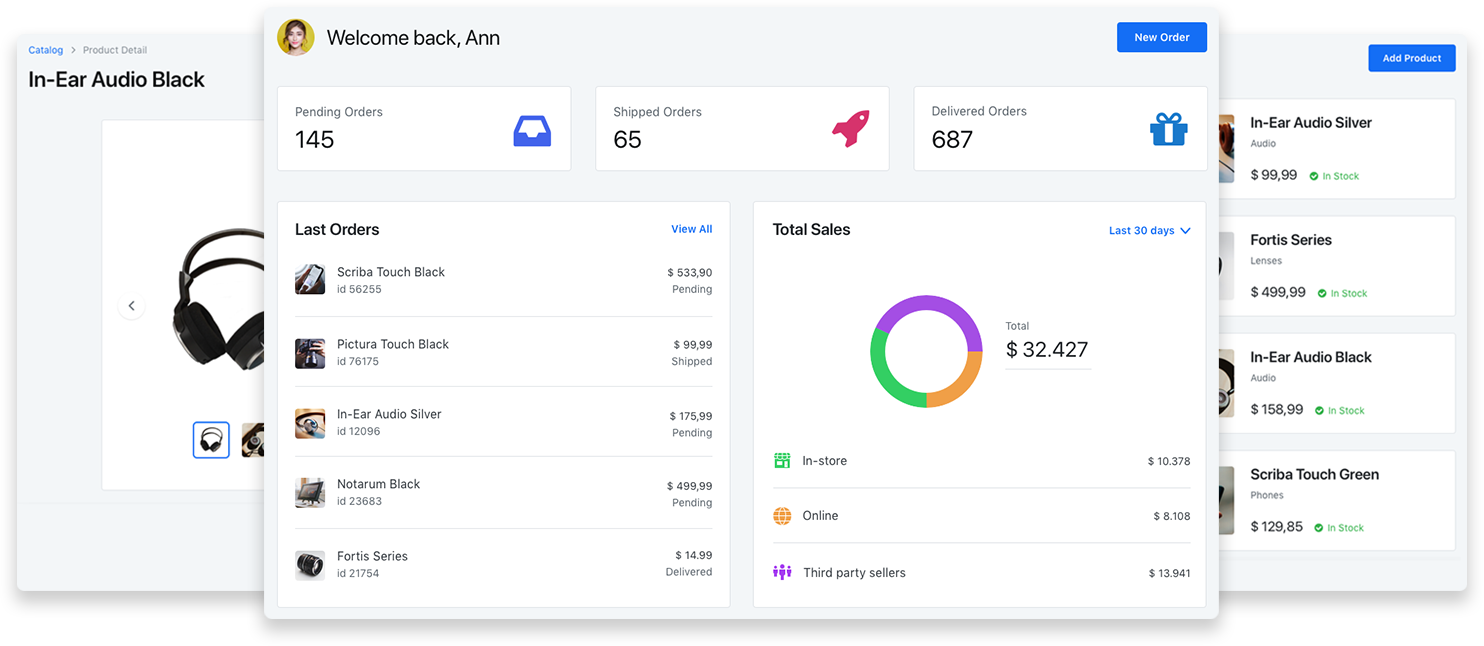
\includegraphics[width=1.0\textwidth]{assets/outsystems-app.png}
\end{frame}
\begin{frame}{\secname}{\subsecname}
  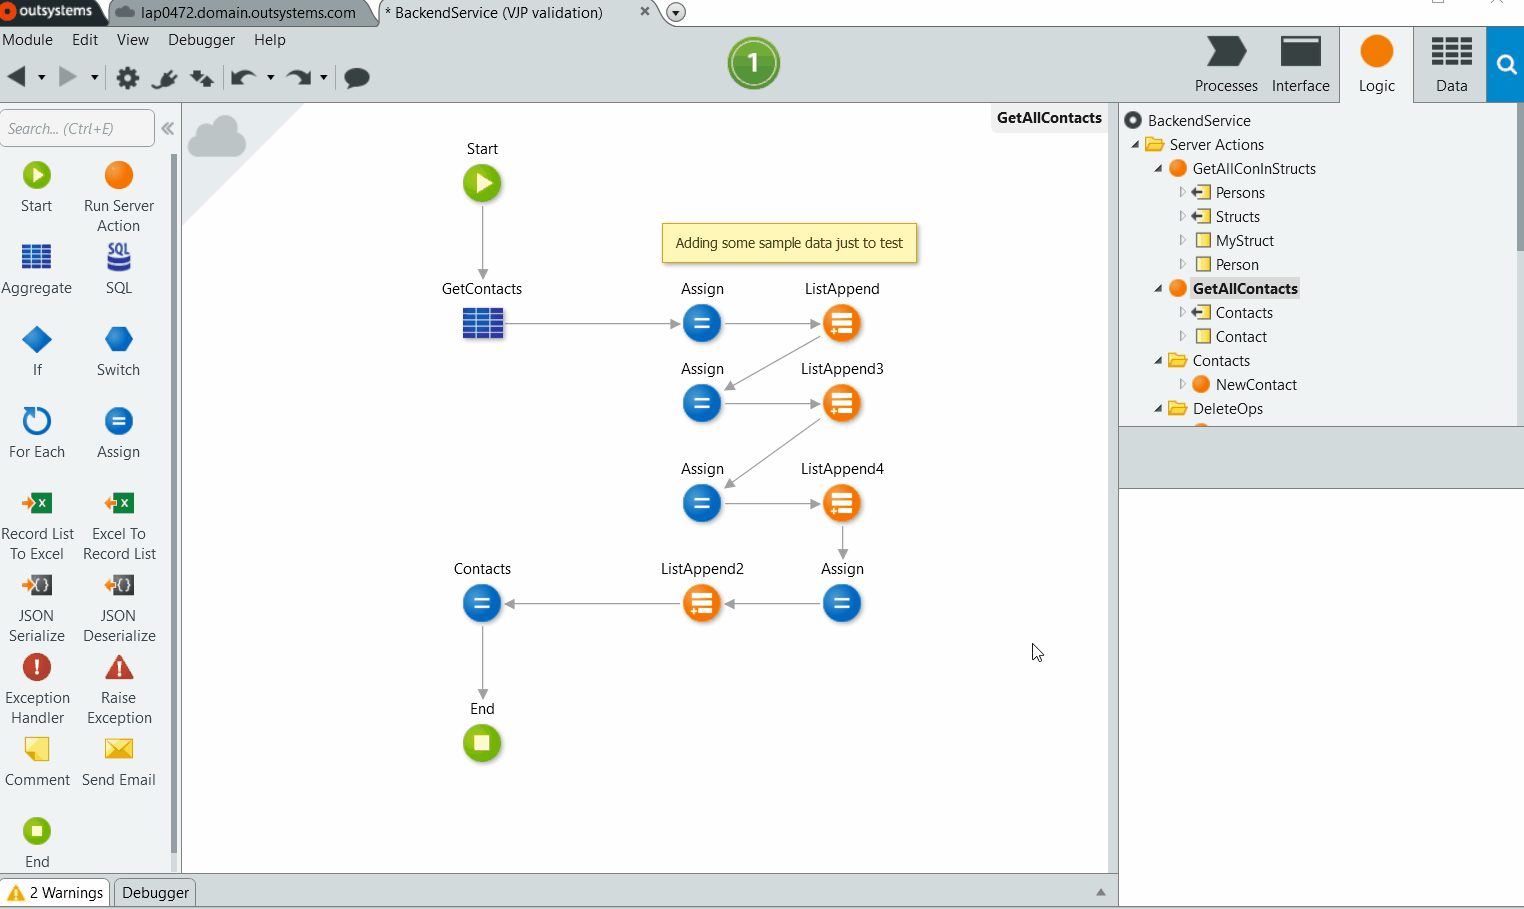
\includegraphics[width=1.0\textwidth]{assets/outsystems-studio.png}
\end{frame}
\begin{frame}[fragile]{\secname}{\subsecname} % 2 mins
  Interested in synthesizing OutSystems expressions:
  
  \begin{itemize}
  \item Small, pure functional language
  \item Builtin functions to manipulate dates, \textbf{text}, \textbf{numbers},
    etc.
  \end{itemize}

($<$"John Michael Doe", "Dr. "$>$, "Dr. John")

\begin{lstlisting}
prog(name, prefix) = Concat(prefix,
                       Substr(name, 0,
                         Index(name, " ", 0)))
\end{lstlisting}
\end{frame}

% ==============================================================================
\section{Synthesis} % 10 mins
\begin{frame}{\secname} % 2 mins
  \begin{itemize}
  \item Component-based
    \begin{itemize}
    \item \lstinline{Concat(t: Text, s: Text)}
    \item \lstinline{Length(t: Text)}
    \item \lstinline{Index(t: Text, s: Text, n: Integer)}
    \item \lstinline{Substr(t: Text, i: Integer, n: Integer)}
    \item \lstinline{Add(x: Integer, y: Integer)}
    \item \lstinline{Sub(x: Integer, y: Integer)}
    \end{itemize}
  \item Programming by examples
  \item Reduction to constraint solving
  \end{itemize}
\end{frame}

\subsection{Constraint Solving}
\begin{frame}{\secname}{\subsecname} % 2 mins
  Reduce the problem to SMT solving.

  \onslide<2->{
  \begin{align*}
  \text{`'Dr. John''} = x \strconcat{} Substr(\text{``John Michael Doe''}, y, z)
  \end{align*}}

  \onslide<3->{
  \begin{align*}
  x = \text{``Dr. ''}, y = 0, z = 4
  \end{align*}}
\end{frame}

\subsection{Setwise Synthesizer}
\begin{frame}{\secname}{\subsecname} % 2 mins
  \begin{figure}[htb]
    \centering
    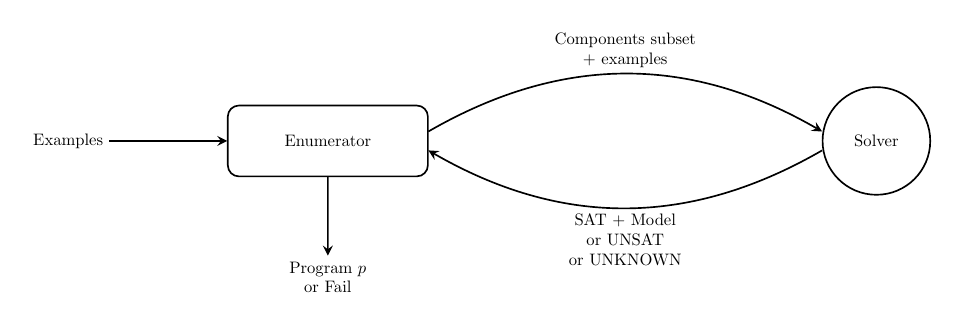
\begin{tikzpicture}
      [semithick, >=stealth, auto,
      rectangular/.style={rectangle, draw, rounded corners, text width=4cm,
        align=center, minimum size=1.5cm},
      spherical/.style={circle, draw, text width=2cm, align=center},
      scale=0.6, every node/.style={scale=0.6}]

      \node [rectangular] (S)  {Enumerator};
      \node [left=1.5cm of S, align=center] (I) {Examples}
      edge [->] (S);
      \node [below=of S, align=center] {Program $p$\\or Fail}
      edge [<-] (S);
      \node [spherical] (V)  [right=5cm of S] {Solver}
      ([yshift=0.2cm]S.east) edge [->, bend left]  node [align=center]      {Components subset\\+ examples}     ([yshift=0.2cm]V.west)
      ([yshift=-.2cm]S.east) edge [<-, bend right] node [swap,align=center] {SAT + Model\\or UNSAT\\or UNKNOWN} ([yshift=-.2cm]V.west);
    \end{tikzpicture}
  \end{figure}
\end{frame}
\begin{frame}[fragile]{\secname}{\subsecname} % 2 mins
\begin{lstlisting}
prog(name, prefix) = Concat(prefix,
                       Substr(name, 0,
                         Index(name, " ", 0)))
\end{lstlisting}
  \begin{columns}
    \begin{column}{0.5\textwidth}
      \begin{lstlisting}
prog(name, prefix):
  c0 = " "
  c1 = 0
  r1 = Index(name, c0, c1)
  r2 = Substr(name, c1, r1)
  r3 = Concat(prefix, r2)
      \end{lstlisting}
    \end{column}
    \onslide<2->{
    \begin{column}{0.47\textwidth}
      $i_0 =$ ``John Michael Doe''

      $i_1 =$ ``Dr. ''

      $o =$ ``Dr. John''

      $c_0 =$ ?, $c_1 =$ ?

      $r_3 = Concat(p_{11}, p_{12})$

      $r_1 = Index(p_{21}, p_{22}, p_{23})$

      $r_2 = Substr(p_{31}, p_{32}, p_{33})$
      
      $l_{i_o}, l_{c_0}, l_{p_{11}}, l_{r_1}, l_o, \ldots$

      $\Psi{} = \exists L,C\ldotp \bigwedge_{(I, o) \in E}\psi{}_{prog}(I, o, C)$
    \end{column}}
  \end{columns}
\end{frame}

\subsection{Whole Synthesizer}
\begin{frame}{\secname}{\subsecname} % 1 min
  \begin{figure}[htb]
    \centering
    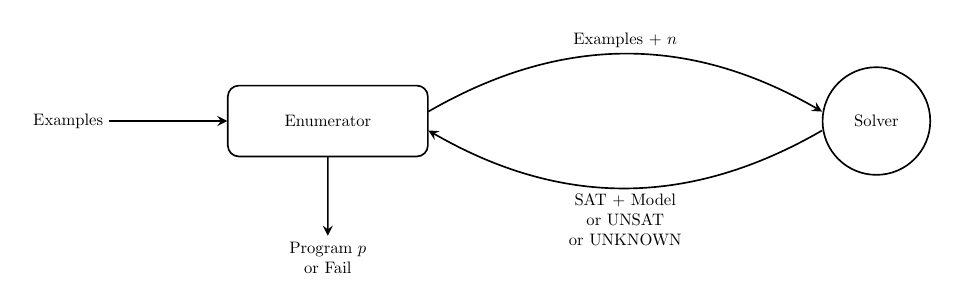
\begin{tikzpicture}
      [semithick, >=stealth, auto,
      rectangular/.style={rectangle, draw, rounded corners, text width=4cm,
        align=center, minimum size=1.5cm},
      spherical/.style={circle, draw, text width=2cm, align=center},
      scale=0.6, every node/.style={scale=0.6}]

      \node [rectangular] (S)  {Enumerator};
      \node [left=1.5cm of S, align=center] (I) {Examples}
      edge [->] (S);
      \node [below=of S, align=center] {Program $p$\\or Fail}
      edge [<-] (S);
      \node [spherical] (V)  [right=5cm of S] {Solver}
      ([yshift=0.2cm]S.east) edge [->, bend left]  node [align=center]      {Examples + $n$}     ([yshift=0.2cm]V.west)
      ([yshift=-.2cm]S.east) edge [<-, bend right] node [swap,align=center] {SAT + Model\\or UNSAT\\or UNKNOWN} ([yshift=-.2cm]V.west);
    \end{tikzpicture}
  \end{figure}
\end{frame}
\begin{frame}[fragile]{\secname}{\subsecname} % 1 min
  \begin{columns}
    \begin{column}{0.5\textwidth}
      \begin{lstlisting}[mathescape=true]
prog($i_0$, $i_1$):
  $c_0$ = ?
  $c_1$ = ?
  $r_1$ = $f_{a_1}$($p_{11}$, $p_{12}$, $p_{13}$)
  $r_2$ = $f_{a_2}$($p_{21}$, $p_{22}$, $p_{23}$)
  $r_3$ = $f_{a_2}$($p_{31}$, $p_{32}$, $p_{33}$)
      \end{lstlisting}
    \end{column}
    \begin{column}{0.5\textwidth}
      \begin{lstlisting}
prog(name, prefix):
  c0 = " "
  c1 = 0
  r1 = Index(name, c0, c1)
  r2 = Substr(name, c1, r1)
  r3 = Concat(prefix, r2)
      \end{lstlisting}
    \end{column}
  \end{columns}
\end{frame}

% ==============================================================================
\section{Experimental Results} % 4 min

\subsection{Description} % 2 mins
\begin{frame}{\secname}{\subsecname}
  \begin{itemize}
  \item 51 expressions drawn from real-world applications
  \item Manually crafted 3 I/O examples for each expression
  \item Tested different configurations, differing on the number of constants
    and examples
  \item 600 seconds, 16 GB, Intel(R) Xeon(R) CPU E5-2620 v4 @ 2.10GHz
  \item Z3 SMT solver version 4.8.5
  \end{itemize}
\end{frame}

\subsection{Results} % 2 mins
\begin{frame}{\secname}{\subsecname}
  In general:
  \begin{itemize}
  \item Less programs found when number of examples is increased, but results
    are more accurate
  \item Worse results when we increase the number of constants (faster, but less
    accurate) 
  \item Mean running time under 60 seconds, median under 10 seconds
  \item Setwise can sometimes synthesize programs up to 3 lines
  \item Whole shows poor results, even for small instances
  \end{itemize}
\end{frame}
\begin{frame}
  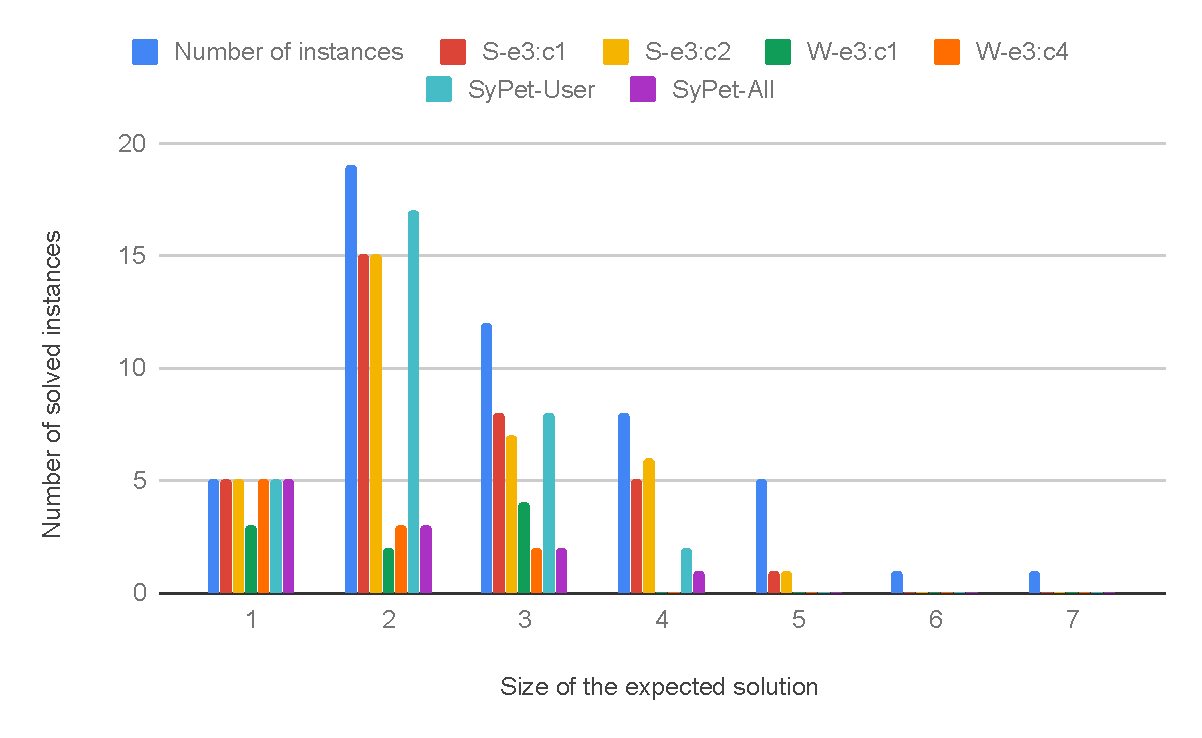
\includegraphics[width=1.0\textwidth]{assets/comparison-solved-sypet-new.pdf}
\end{frame}
\begin{frame}
  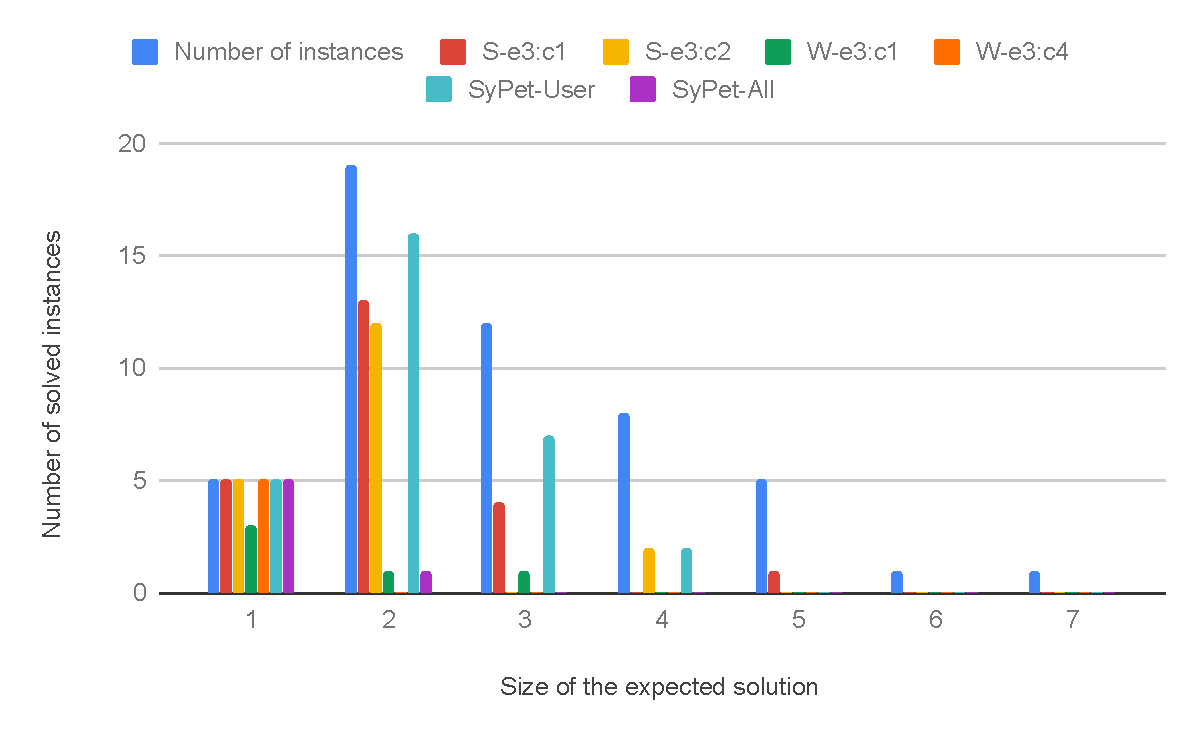
\includegraphics[width=1.0\textwidth]{assets/comparison-expected-sypet-new.pdf}
\end{frame}

% ==============================================================================
\section{Conclusion and Future Work} % 2 min
\begin{frame}{\secname}
  \begin{itemize}
  \item Developed two synthesizers based on constraint-solving for a subset of
    OutSystems
  \item Not practical right now, works only for very small instances, even with
    a small library of components
  \item It would be interesting to check the effects of some tweaks. For example: 
    \begin{itemize}
    \item Applying restrictions to the values of the constants
    \item Adding templates
    \item Accepting user-defined constants
    \end{itemize}
  \end{itemize}
\end{frame}

\end{document}
